\chapter{Kiértékelés}
\label{sec:kiertekeles}

Ebben a fejezetben a programom tesztelését mutatom be. Az első alfejezetben (\ref{sec:kiertekeles_teszt}) a tesztelés részleteiről írok, a második alfejezetben (\ref{sec:kiertekeles_ered}) az elért értékelem ki a harmadik alfejezetben (\ref{sec:osszesites}) pedig összesítem a futtatások eredményeit.

\section{Tesztelés}
\label{sec:kiertekeles_teszt}
A programom készítése közben folyamatosan teszteltem azt JUnit tesztek segítségével az Architektúra (\ref{sec:architektura}) alfejezetben bemutatott \texttt{CfaTest} osztállyal. A tesztekhez a CFA modelleket egyrészt az \texttt{ftsrg} kutatócsoport \texttt{ca} github repository-jából nyertem \cite{ca-lab-tests}, illetve készítettem sajátokat is, de a tesztek túlnyomó többsége a Thetához kapcsolódó, privát GitHub repository-ból való, amelyek különböző frontendekkel lettek generálva. Az utóbbiban többek között 479 darab CFA teszt található, melyekhez tartozik előre ismert eredmény is. A tesztek egyik fele az SV-Comp-ról\footnote{\url{https://sv-comp.sosy-lab.org/2018/}} származik ahol eredetileg C kódok voltak, amik aztán át lettek CFA-ba alakítva \cite{vpt2017}. Ezek különböző csoportba sorolhatóak \cite{akos-phd}:

\begin{itemize}
	\label{felsorolas}
	
	\item \texttt{Locks} kicsi (94-234 LoC\footnote{Source lines of code - Hány sorból áll a program melyet a CFA modellez.}) kizárási feladatokat ír le.
	
	\item \texttt{ECA} (event-condition-action) feladathalmaz nagy (591-1669 LoC) eseményvezérelt rendszereket tartalmaz.
	
	\item \texttt{SSH} nagy (557-716 LoC) kliens-szerver rendszereket ír le.
	
	\item \texttt{Simple} kicsi (14-40 LoC) feladatok gyors teszteléshez.
\end{itemize}
\ \\
Továbbá volt alkalmam tesztelni olyan CFA modelleket is, melyek eredetileg ipari PLC szoftverkódok voltak a CERN-nél. \cite{darvas2019plcverif} Ezek mérete roppant változatos -- a pár tucattól a több ezerig is terjedhet. Mindegyik tesztről tudjuk, hogy abban mennyi változó van (azok között mennyi int és mennyi boolean típusú), mennyi hely, mennyi él, az egyes taszkok ciklikus komplexitása, az éleken mennyi hozzárendelés, mennyi őrfeltétel illetve hogy mennyi havoc van. Ezeket vázlatosan bemutatja a (\ref{table:tasksStat}) táblázat \cite{akos-phd}:

\begin{table}[h] 
	\centering
	\begin{tabular}{lllllll}
		\toprule
		Category & Tasks & Vars & Locs & Edges & CC\\
		\midrule
		Simple & 10 & 1--2 & 4--12 & 3--13 & 3--9\\
		Locks & 143 & 4--32 & 9--40 & 10--57 & 3--23\\
		SSH & 17 & 64--81 & 187--267 & 262--375 & 87--121\\
		PLC & 129 & 1--596 & 8--4614 & 7-4782 & 4-188\\
		ECA & 180 & 9--30 & 302--1301 & 375--1516 & 73--231\\
		
		\bottomrule
		\textit{Total} & \textit{479}\\
	\end{tabular}
	\caption{Az egyes taszkok tulajdonságainak statisztikai jellemzői. A CC rövidítés a Cyclomatic Complexity azaz a ciklikus komplexitást jelöli.}
	\label{table:tasksStat}
\end{table}
\ \\
Míg a program fejlesztése közben azt 28 darab, véletlenszerűen kiválasztott teszttel ellenőriztem, a végén teszteltem mind a 479 tesztre is. A széleskörű teszteléshez a \texttt{KInductionCLI} osztályt használtam, mely egy interfészt biztosít a programom parancssori futtatásához, és amelyet a következő paraméterekkel lehet meghívni:

\begin{itemize}
	\item \texttt{-{}-model} -- A CFA teszt elérési útvonala, ha csak egy darab tesztre szeretnénk lefuttatni. Nem kötelező.
	\item \texttt{-{}-input} -- A CFA teszteket, az elvárt eredményeiket és egyéb, a tesztek tulajdonságait leíró információkat tartalmazó .csv fájl elérési útvonala. Nem kötelező.
	\item \texttt{-{}-time} -- A futási időt tudjuk vele korlátozni, másodpercben. Nem kötelező, alapértelmezetten -1.
	\item \texttt{-{}-bound} -- Az algoritmus bejárási mélységét tudjuk vele korlátozni. Nem kötelező, alapértelmezetten -1.
	\item \texttt{-{}-output} -- A kimenetel fájl neve (input paraméter esetén). Nem kötelező, alapértelmezetten ``output.csv''.
\end{itemize}
Habár se a \texttt{-{}-model} sem az \texttt{-{}-input} paraméter nem kötelező, a program \texttt{assert}-tel ellenőrzi, hogy legalább egy meg legyen adva. Viszont ugyanúgy hiba, ha kettő bemenet van adva. Ezt az alábbi kóddal ellenőrzöm:
\ \\
\begin{lstlisting}
	if (!input.equals("") && !model.equals("")) {
			Assert.fail("Only one input source is allowed.");
	}
	if (input.equals("") && model.equals("")) {
			Assert.fail("One input source is required.");
	}
\end{lstlisting}

\section{Eredmények}
\label{sec:kiertekeles_ered}

Azon teszteknél, melyekre a programom készítése közben azt folyamatosan teszteltem, az ideális ellenpéldahossz is meg volt adva. A programom kivétel nélkül mindre (11 darab) az optimális megoldást produkálta. 
\\
\\
A 479 tesztet az előző oldalon található felsorolás szerint külön .csv fájlokba szerveztem. Ezután a 
\ \\
\begin{lstlisting}
	java -jar theta-k-induction.jar --input input_xx.csv --output output_xx_yy.csv --time yy
\end{lstlisting}
\ \\
parancssori utasítást adtam ki, ahol xx = \{locks, eca, ssh, simple, plc\}, illetve yy = \{60, 120, 180, 300, 600\}, azaz szavakkal elmondva külön-külön mindegyik tesztkategóriát futtattam 1 perc, 2 perc, 3 perc, 5 perc illetve 10 perc időkorláttal. Azért döntöttem időkorlát használata mellett, mert tapasztalataim szerint egyes tesztek 8, 10 vagy annál több óra futási időt is igényelhetnek, ami a nagy darabszámot is figyelembe véve korlátozásra ad okot. 

A parancssori interfészről készítettem képeket, melyek megtekinthetők a Függelékben (\ref{sec:parancs_int_fel}). Itt a harmadik ábra (\ref{fig:cli_3}) külön érdekes: a program futása után statisztikát közlök arról, hogy hány teszt lett sikeres, mennyi nem sikerült azért, mert ismeretlen lett és mennyi nem sikerült azért, mert tévedett a programom. Ez az utóbbi minden futtatásnál \textbf{0} volt.
\\
\\
A kapott eredményfájlokat a Pandas\footnote{\url{https://pandas.pydata.org/}} Python programkönyvtárral dolgoztam fel. A következő eredményekre jutottam:

\begin{itemize}
	\item Azt tapasztaltam, hogy a tesztek 64.3\%-a lett biztonságos, 9.39\%-a lett nem biztonságos és 26.3\%-a lett ismeretlen.
	\item Viszont arra lettem figyelmes, és ez az (\ref{fig:rec_rate_during_time}) ábrán jól is látszik, egyes tesztkategóriákban 100\% felismerési arányt sikerült elérni.
\end{itemize}

A felismerési arány alatt azt értem, hogy az adott kategóriában a tesztek hány százaléka lett nem ismeretlen, tehát a tesztek hány százalékát láttuk be. Szeretném kihangsúlyozni, hogy minden egyes tesztre, ami nem ismeretlen lett, \textbf{helyes} választ adott a programom. Néhány nagyobb, bonyolultabb tesztnél engedtem végig futni (a statisztikában nem szerepelnek), és azokra is mind \textbf{helyes} eredményt kaptam, így arra jutottam, hogy a korlátozás nem befolyásolja a programom működését, annak csak időmenedzsmenti okai és következményei vannak.
\\
\begin{figure}[!ht]
	\centering
	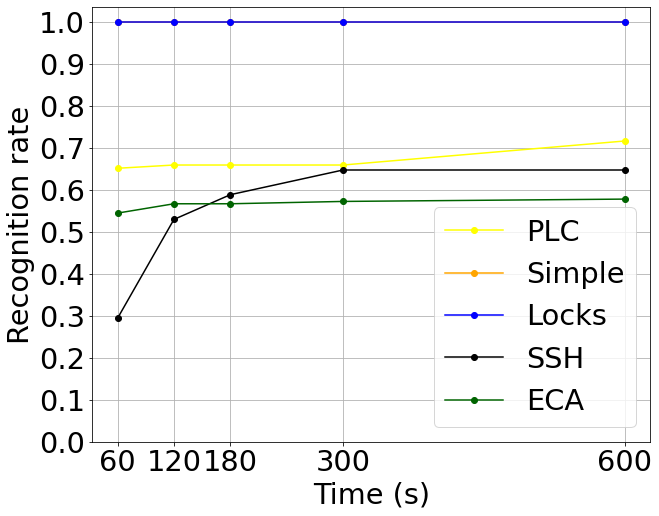
\includegraphics[width=100mm, keepaspectratio]{figures/fig_rec_rate_during_time.png}
	\caption{A tesztek felismerési arányainak a változása különböző időkorlátokkal futtatva. A Simple végig 100\%-os felismerési arányt produkált, mint a Locks, csak az utóbbi kitakarja az ábrán.}
	\label{fig:rec_rate_during_time}
\end{figure}

\clearpage

A fejezet maradék részében a futtatási eredményeket fogom elemezni, hogy a tesztek egyes tulajdonságai hogyan hatnak ki a futási időre. A futtatásokat elemző képek a Függelék Teszteredmények (\ref{sec:fug_teszt_ered}) alfejezetében találhatóak. Mindegyik képen az X tengely a tesztek egy adott tulajdonsága látható, az Y tengelyen pedig a futási idő az adott tulajdonságra vetítve másodpercben. Mindegyik kép a 10 percig futtatott program eredményeit mutatja, azért, hogy a lehető legtöbb információt tudjam megjeleníteni.
\\
\\
A 100\%-os felismerési arány a Simple és a Locks kategóriák esetén nem meglepő, ha ránézünk a (\ref{fig:locks}) ábrára. Látható, hogy másodpercek alatt képes volt a programom ellenőrizni a modelleket, így még csak közel sem került az időkorláthoz.

Az (\ref{fig:rec_rate_during_time}) ábrán látható, hogy az SSH tesztkategóriának az egyperces futási idő kevés, viszont ahogy emeljük a korlátot, úgy nő a sikeresen lefutott tesztek száma. Egészen öt percig, ahol is megtorpanni látszik: nem változik utána a felismerési arány. Öt percig az eredmény 3 biztonságos, 8 nem biztonságos és 6 ismeretlen, és hiába emeltük a duplájára az időkorlátot, a maradék 6 ismeretlenből egyiket se sikerült belátni. 

Az (\ref{fig_ssh_a}) ábrán a következőt láthatjuk: a változók számától önmagában egyedül biztosan nem függ a futási idő, tekintve, hogy volt olyan teszteset ahol 81 változóval a program 23 másodpercig futott illetve 78 változóval 42 és 45 másodpercekig, míg 77 változóval rendre (hatszor) túllépte a 600 másodperces időkorlátot. Tehát kell lennie legalább még egy tulajdonságnak, amivel együtt határozzák meg a tesztek futási idejét.
\\
\\
Az (\ref{fig_plc}) ábrán láthatjuk a PLC tesztkategória eredményeit. Fontos megjegyezni, hogy PLC tesztből közel 8x annyi állt rendelkezésre, mint SSH-ból, így a következő eredmények biztosan pontosabban fogják leírni a tesztek szórását. Az láthatóan kijelenthető, hogy nagy (változó, él, hely illetve komplexitás) értékekre a futásidő nem fog beleférni a 10 perces korlátba. Érdemes megfigyelni az ábrák elején lévő pont-sűrűsödést, amik alapján elmondható, hogy alacsony paraméterek mellett (Vars < 60, Edges < 150, Locs < 150, CC < 25) a programom nagy valószínűséggel fut le 10 percen belül. 
\\
\\
Az ECA tesztkategóriánál az (\ref{fig_eca}) ábrán a kétpóluság figyelhető meg: az ábrák négy sarkaiban jelennek meg a futtatások eredményei, tehát vannak tesztek amik kevés változó / él / hely mellett gyorsan lefutottak de olyanok is amik túllépték az időkorlátot, illetve vannak tesztek melyek sok változó / él / hely esetén néhány pár másodperc alatt lefutottak, a többi meg túllépte az időkorlátot. A komplexitást mutató (\ref{fig_eca_cc}) ábra nem közöl sok új információt, csupán annyit, hogy minél kisebb, annál nagyobb az esélye, hogy időben lefut -- viszont ez az esély nem sokkal nagyobb.

\clearpage

\section{Összesítés}
\label{sec:osszesites}

Megállapítható, hogy az esetek többségében a kisebb  \{változó, él, hely\} szám illetve komplexitás érték gyorsabb futási időt jelent, ahogy az várható is volt, viszont sok esetben pont ennek az ellentette látszik. Úgy láttam, nem lehet egyértelműen kijelenteni, hogy a futási idő melyik paramétertől függ, az sokkal inkább a tesztfelépítésétől függ: ha az állapottér kifejtése során nagy végtelen ciklusba kerülünk már az elején, akkor azt a program végéig fogjuk megállás nélkül körbe fejteni, illetve közben az állapottér újabb és újabb szintjeit fedezzük fel, így azokat is ki kell minden egyes körben mellé fejteni. Ez nagyon sok erőforrást lefoglal és lassú lesz a bejárás.

Ezzel szemben míg ha sok változót, helyet illetve élet is tartalmaz a teszt, de nem található benne nagyobb végtelen kör, a bejárás gyors lesz és a program le fog tudni futni az időkorláton belül.